\documentclass[conference]{IEEEtran}

% ------------------------------------------------------------
% Packages
% ------------------------------------------------------------
% T1 is required: the bibliography contains an ogonek (M\k{a}dry), which OT1 cannot set.
\usepackage[T1]{fontenc}
\usepackage{amsmath,amssymb,amsfonts}
\usepackage{algorithm}
\usepackage{algorithmic}
\usepackage{array}
\usepackage{booktabs}
\usepackage{graphicx}
\usepackage{textcomp}
\usepackage{xcolor}
\usepackage{url}
% hidelinks: without it every \ref, \cite and \url is drawn with a colored border box,
% which is distracting in the requirement tables where rule ids are set with \url.
\usepackage[hidelinks]{hyperref}
\usepackage{multirow}
\usepackage{enumitem}

% Verbatim listings used by the worked examples in Sections I, IV and V.
\usepackage{fancyvrb}
\usepackage{framed}

% ------------------------------------------------------------
% Paper information
% IMPORTANT:
% IPDPS 2027 uses double-anonymous review.
% Do not include author names, affiliations, or identifying
% information in the submission version.
% ------------------------------------------------------------

\title{Evaluating LLM Agents for Autonomous Scientific Workflows on HPC Systems}

% Anonymous submission:
% \author{
% \IEEEauthorblockN{Anonymous Authors}
% }

\begin{document}

\maketitle

% ------------------------------------------------------------
% Abstract
% ------------------------------------------------------------


\begin{abstract}
Large language model (LLM) agents are increasingly proposed for automating scientific workflows, but executing a scientific application on a supercomputer requires satisfying scientific and system constraints \emph{simultaneously}: an application that is scientifically appropriate may not be installed on the target machine, and a correctly prepared input may be paired with resources its parallel execution model cannot use. We present \textit{Trinity}, a multi-agent framework for autonomous scientific discovery on high-performance computing (HPC) systems, together with a benchmark for the capability the rest of the framework depends on---constructing a valid workload before submission. The benchmark covers four subtasks (software selection, input preparation, resource selection, and batch-job creation) over ten application/system anchors spanning seven supercomputers and two schedulers. Because multiple solutions can be valid, responses are graded by a versioned library of 56 requirements mined from 138 archived production runs rather than by similarity to a reference answer; where successful runs disagree with one another, the disagreement is recorded as \emph{free choice} that the judge may not penalize. Evaluating four open-weight models with and without facility knowledge in the prompt, pass rates rise from 27/160 to 99/160. On the subset of requirements registered \emph{before} the run as satisfiable without the injected facts, the same augmentation yields 87/160 to 119/160, separating what the models learned from what the prompt supplied.
\end{abstract}

\begin{IEEEkeywords}
HPC, autonomous scientific discovery, scientific workflows,
LLM agents, high-performance computing, agentic systems
\end{IEEEkeywords}

\section{Introduction}\label{sec:introduction}

Large language models (LLMs) are increasingly being developed as agents that reason about complex tasks, invoke external tools, observe the resulting environment, and iteratively determine subsequent actions. This capability creates new opportunities for automating scientific workflows, where progress from a scientific question to a result requires a sequence of computational and reasoning steps rather than a single program or answer: an agent may need to identify an appropriate scientific method, prepare inputs, execute computations, inspect results, diagnose failures, and decide what to do next. Recent scientific-agent research has begun to automate substantial portions of this process while also highlighting the need for rigorous evaluation of individual capabilities before making claims about end-to-end scientific automation~\cite{chen2025scienceagentbench}. High-performance computing (HPC) is the infrastructure on which such workflows run at scale, and it introduces constraints that an autonomous agent must satisfy before any of its decisions can be executed.

The central difficulty is that scientific HPC workflows require reasoning across two tightly coupled sources of context. The \textit{scientific application context} comprises application semantics, input formats, scientific parameters, execution models, and dependencies. The \textit{HPC system context} comprises hardware architecture, installed software, scheduler policies, queue limits, filesystems, and site-specific execution procedures. These cannot be treated independently: the application constrains which inputs and execution strategies are meaningful, while the target system constrains which implementations and resources are feasible. An agent can therefore hold correct knowledge of either domain and still produce an unusable workflow---selecting a scientifically appropriate application that is not installed, preparing a valid input but requesting resources incompatible with its parallel execution model, or writing a syntactically valid batch script that does not connect the chosen application, inputs, and resources. The problem is thus neither resource management nor code generation, but \emph{cross-domain constraint satisfaction}.

\begin{figure*}[t]
\centering
\begin{minipage}[t]{0.48\textwidth}
\textbf{(a) Without facility context.} The agent is told the workload, the
working directory, the resources, and the account.
\begin{Verbatim}[fontsize=\scriptsize,frame=single,framesep=2mm]
#!/bin/bash
#PBS -N lammps_argon_500k
#PBS -l select=1:ncpus=32:mpiprocs=4
#PBS -l walltime=00:30:00
#PBS -q debug
#PBS -A TrinityAgent
#PBS -o /eagle/.../lammps_run/output/lammps.out
#PBS -e /eagle/.../lammps_run/error/lammps.err
...
module use /soft/modulefiles
module load lammps
mpiexec -n 4 lmp -in in.lammps
\end{Verbatim}
\emph{Judge (all three replicates): \textbf{fatal}.}
``The script has no \verb|#PBS -l filesystems=...| directive despite
accessing \verb|/eagle/...| paths.''\\[2pt]
Everything else is right---job name, queue, walltime, account, output
paths, working directory, launcher. The job would be rejected or hang.
\end{minipage}\hfill
\begin{minipage}[t]{0.48\textwidth}
\textbf{(b) With facility context.} The same model, same workload; the
prompt now carries the site's scheduler conventions.
\begin{Verbatim}[fontsize=\scriptsize,frame=single,framesep=2mm]
#!/bin/bash -l
#PBS -l select=1:system=polaris
#PBS -l place=scatter
#PBS -l walltime=00:30:00
#PBS -l filesystems=home:eagle
#PBS -q debug
#PBS -A TrinityAgent
...
module load PrgEnv-gnu
module swap gcc-native gcc-native/12.3
module load cray-mpich
export PATH=/eagle/.../lammps/bin:$PATH
mpiexec -n ${NTOTRANKS} --ppn 4 lmp -in in.lammps ...
\end{Verbatim}
\emph{Judge (all three replicates): \textbf{no requirement violated}.}
``Includes \verb|#PBS -l filesystems=home:eagle|, covering the Eagle
working directory and binary path.''\\[2pt]
The invented \verb|module load lammps| is also replaced by the real
build's module stack.
\end{minipage}
\caption{The capability gap is often a single site-specific fact, not a
reasoning failure. Both scripts were produced by Nemotron-3-Ultra for the
same LAMMPS workload on Polaris. The augmented prompt adds, among other
material, one line of site convention: \emph{``ALCF requires \texttt{\#PBS
-l filesystems=<list>} naming every filesystem the job touches
(Polaris/Crux/Sophia: \texttt{home:eagle}) or the job is rejected or
hangs.''} This single requirement,
\texttt{BATCH.common.filesystems\_declared}, is violated in 31 of 40
unaugmented batch-job instances and in none of the augmented ones.}
\label{fig:motivating-example}
\end{figure*}

Figure~\ref{fig:motivating-example} shows what this looks like in practice, and why it is easy to
mistake for competence. Asked to write a batch script for a 500,000-atom LAMMPS simulation on
Polaris, a strong open-weight model produces a script that is correct in every visible
respect---job name, queue, walltime, charge account, output paths, working directory, and
launcher---and is nonetheless rejected by the scheduler, because it omits the
\texttt{filesystems=} directive that this facility requires and few others do. The missing line is
not a reasoning error. It is a fact about one site, unknowable from pre-training, and no amount of
additional deliberation would recover it. Supplying that convention in the prompt eliminates the
violation across all 40 batch-job instances. Distinguishing this kind of failure from a genuine
capability gap is the central measurement problem this paper addresses, and it is why our
evaluation reports what the prompt supplied separately from what the model knew.

Evaluating the capability presents three further difficulties. First, these tasks have no single
correct answer: many applications, resource configurations, and scripts can satisfy the same
objective, so textual similarity to a reference is not a correctness signal. Second, the artifacts
are coupled---a wrong application invalidates the inputs, and an inconsistent
application/input/resource triple yields an invalid job---so grading only the final artifact hides
where the agent actually failed. Third, deciding correctness requires domain knowledge of both
application semantics and the target system. Together these motivate an evaluation that decomposes
workflow construction into subtasks while preserving the dependencies among their constraints.

We present \textit{Trinity}, a multi-agent framework for autonomous scientific discovery and
execution across HPC environments. Trinity enables LLM-based agents to turn high-level scientific
objectives into executable workflows, interact with scientific applications and HPC infrastructure,
observe results, and use those observations to choose subsequent actions; a complete workflow
extends beyond submission to data and environment preparation, monitoring, failure diagnosis and
recovery, result analysis, and reporting. This paper focuses on the capability the rest of that
vision presupposes: constructing a valid scientific HPC workload in the first place. We evaluate it
through the four pre-submission stages---software selection, input preparation, resource selection,
and batch-job creation---which together capture the decisions that translate scientific intent into
an executable job, in a setting controlled enough to localize where and why agents fail.

Our contributions are as follows:
\begin{itemize}
\item \textbf{Trinity framework for autonomous scientific discovery.} A multi-agent framework connecting LLM-based reasoning with scientific applications, HPC systems, data-management services, execution infrastructure, monitoring, and scientific feedback to support iterative scientific workflows.

\item \textbf{Scientific HPC workflow benchmark.} A benchmark covering four pre-submission capabilities---software selection, input preparation, resource selection, and batch-job creation---over ten application/system anchors spanning seven supercomputers and two schedulers, explicitly capturing the coupled constraints between scientific applications and HPC environments.

\item \textbf{Constraint-based and domain-aware evaluation.} A versioned library of 56 requirements, each carrying its provenance, that evaluates candidate solutions by constraint satisfaction rather than similarity to a reference answer. Requirements are mined from archived production runs and revised through human review, and disagreement among successful runs is recorded as \emph{free choice} the judge may not penalize.

\item \textbf{Separating supplied knowledge from model capability.} We measure inference-time capability augmentation against a knowledge-dependence classification of every requirement, registered before any answer was collected, so that gains attributable to facts the prompt supplied are reported separately from gains in what models can do unaided.
\end{itemize}

\section{Background and Related Work}\label{sec:related}

\subsection{AI Agents}

LLM-based agents reason about tasks, invoke external tools, and act on resulting observations, following the interaction pattern established by ReAct~\cite{yao2023react} and extended by multi-agent orchestration frameworks such as AutoGen~\cite{wu2024autogen}. Other work augments agents with externally maintained skills and knowledge without modifying model parameters. For example, Voyager maintains an executable skill library and improves it through environmental feedback~\cite{wang2023voyager}. This separation between model parameters and externally supplied knowledge is particularly relevant to scientific computing, where facility-specific software, system configurations, and application knowledge can change over time. Scientific HPC agents therefore require not only general agentic reasoning and tool use, but also reasoning over application semantics, input requirements, system architecture, software availability, scheduler policies, resource limits, and execution procedures.

\subsection{Scientific and HPC Agents}

Recent work applies LLM agents to scientific and HPC workflows. Ma et al.\ integrate Parsl with LangChain/LangGraph so an LLM agent can invoke scientific tools distributed across HPC resources, demonstrating molecular-dynamics workflows on Polaris~\cite{ma2025langchainparsl}. Diamond Agent instead focuses on workload placement across heterogeneous, independently administered supercomputers using live system and queue information~\cite{diamondagent2026}. Other work studies agents for workflow provenance~\cite{souza2025provenance}, while ECAS separates agent reasoning from execution-side control so that proposed artifacts can be validated before production execution~\cite{sun2026ecas}. These systems primarily focus on executing, orchestrating, placing, or validating workflows, whereas Trinity evaluates whether an agent can \textit{construct} a valid workflow from a high-level objective.

Closest in motivation is AskHPC, a retrieval-augmented question-answering chatbot for HPC user support built on a curated knowledge base of facility user guides, scheduler manuals, and programming documentation~\cite{bondapalli2025askhpc}. It makes the same diagnosis that motivates our augmented arm---that general-purpose models fail on facility-specific tasks because the necessary facts are scattered, site-specific, and absent from pre-training---and addresses it by supplying retrieved documentation at inference time~\cite{lewis2020rag}. The two efforts are complementary and differ in what is being produced and measured. AskHPC answers a user's question and is evaluated on the accuracy and relevance of that answer; Trinity evaluates whether an agent can construct the executable artifacts of a workload, graded against constraints rather than against reference text. The relationship is also methodological: because supplying documentation is precisely the intervention such systems perform, a benchmark measuring its effect must be able to distinguish improvement in the model's capability from the prompt simply carrying the answer, which is what the knowledge-dependence split in Section~\ref{sec:knowledge-split} is for.

Related work also generates or transforms individual HPC artifacts. ParEval evaluates LLM-generated parallel programs across programming models~\cite{nichols2024pareval}, while HPC-Coder and HPC-Coder-V2 develop models specialized for parallel and scientific computing~\cite{nichols2024hpccoder,chaturvedi2025hpccoderv2}. Sochat and Milroy study translation between Slurm and Flux job specifications~\cite{sochat2026descriptive}. Trinity considers a different artifact-construction problem: selecting an application, preparing its inputs, selecting appropriate resources, and constructing a batch-job specification for a target system. These decisions are coupled because correctness depends simultaneously on the \textit{scientific application context} and the \textit{HPC system context}. An application may be scientifically appropriate but unavailable on the target system, or a system-valid resource configuration may be incompatible with the application's requirements. Trinity therefore treats workflow construction as a \textit{cross-domain constraint-satisfaction problem}.

\subsection{Agent Benchmarks and Evaluation}

General-purpose agent benchmarks establish the importance of evaluating agents through realistic interactions and task outcomes. AgentBench evaluates multi-turn decision-making across interactive environments~\cite{liu2023agentbench}, WebArena evaluates action sequences that change and verify environment state~\cite{zhou2024webarena}, and SWE-bench evaluates repository-level code changes through executable tests~\cite{jimenez2024swebench}. Domain-specific benchmarks extend this methodology to engineering and scientific tasks: MLE-bench evaluates ML engineering~\cite{chan2025mlebench}, MLAgentBench evaluates ML experimentation as a sequence of research actions~\cite{huang2024mlagentbench}, and ScienceAgentBench evaluates scientific discovery through generated programs and expert-informed judgments~\cite{chen2025scienceagentbench}. PaperBench evaluates research-paper reproduction through fine-grained rubric-based subtasks and artifact execution~\cite{starace2025paperbench}.

Several benchmarks further demonstrate the value of decomposing complex agent tasks into intermediate capabilities. AgentBoard evaluates progress against explicit subgoals~\cite{ma2024agentboard}, while CORE-Bench uses multiple levels of computational reproducibility~\cite{siegel2024corebench}. SUPER similarly separates individual research subtasks from end-to-end execution and shows that success on individual components does not necessarily imply successful composition~\cite{bogin2024super}. Trinity applies this stage-decomposed perspective to scientific-HPC workflow construction, using distinct artifacts---application selection, input preparation, resource selection, and batch-job creation---rather than trajectory checkpoints.

A key difference is that Trinity's artifacts generally do not have a single executable oracle or reference answer. Multiple applications, resource configurations, and batch scripts may satisfy the same scientific objective. Trinity therefore uses requirement-level domain-aware judging rather than exact matching or a single reference. This builds on LLM-as-judge approaches such as MT-Bench and G-Eval~\cite{zheng2023mtbench,liu2023geval}, rubric-based evaluation such as Prometheus 2~\cite{kim2024prometheus2}, and decomposed evaluation criteria in InFoBench and PaperBench~\cite{qin2024infobench,starace2025paperbench}. Trinity maintains a reusable, versioned requirement library whose criteria are iteratively refined through human review, allowing the benchmark to evaluate correctness consistently across different valid solutions.

\subsection{Scientific and HPC Agent Benchmarks}

AOBench is particularly relevant as an HPC-specific agent benchmark. It evaluates AI agents on operational tasks including job scheduling, telemetry, energy reasoning, and policy enforcement through execution traces in deterministic environments~\cite{aobench}. AOBench therefore evaluates an agent as an \textit{HPC operator} that observes and manipulates facility state under operational and authorization constraints. Trinity instead evaluates an agent as a \textit{scientific workload user}: given a high-level objective, the agent must construct an executable workload by jointly reasoning about the scientific application and the target HPC system. Thus, AOBench emphasizes correct interaction with an existing HPC environment, whereas Trinity emphasizes correct construction of the workload that will be executed in that environment.

This distinction also motivates Trinity's inference-time capability augmentation experiments. Because each workflow-construction subtask exposes a different combination of scientific and system knowledge, the benchmark can investigate whether failures arise from missing application knowledge, missing HPC-system knowledge, insufficient examples, or reasoning limitations. Trinity can then evaluate whether externally supplied knowledge, examples, or other inference-time mechanisms improve these capabilities without modifying model parameters.

Overall, existing work establishes agentic reasoning and tool use, scientific program generation, HPC-resource orchestration, stage-decomposed evaluation, and LLM-as-judge methodology as important but largely separate lines of progress. Trinity addresses the complementary problem of evaluating whether an agent can jointly reason about a scientific application and a target HPC system to construct a workflow that is scientifically valid, system-valid, and executable. It combines \textit{cross-domain workflow evaluation}, \textit{domain-aware judging}, and \textit{inference-time capability augmentation} within a single benchmark.


% ============================================================
\section{Trinity System Overview}
% ============================================================

\subsection{Trinity Overview}

Trinity is a multi-agent, LLM-driven framework for autonomous
scientific discovery and execution. It enables AI agents to
transform high-level scientific objectives into executable
workflows and carry them out across high-performance computing
(HPC) environments. Rather than using an LLM solely for question
answering or code generation, Trinity integrates LLM-based
reasoning with scientific software, HPC execution services,
data-management tools, and system- and application-level
observations. This integration allows agents to plan experiments,
interact with remote computing resources, monitor execution,
analyze results, and determine subsequent actions throughout the
scientific workflow.

Trinity is designed to operate across large-scale computing
environments, including DOE leadership-class supercomputers such
as Polaris, Aurora, Frontier, and Perlmutter. It integrates with
HPC and scientific infrastructure, including data-transfer
services such as Globus and execution interfaces such as IRI and
Globus Compute, enabling agents to work with distributed data,
computational resources, and scientific applications. Through
this integration, Trinity supports scientific workflows in domains
including physics, materials science, chemistry, and astrophysics.


\subsection{Trinity Workflow}

\begin{figure*}[t]
    \centering
    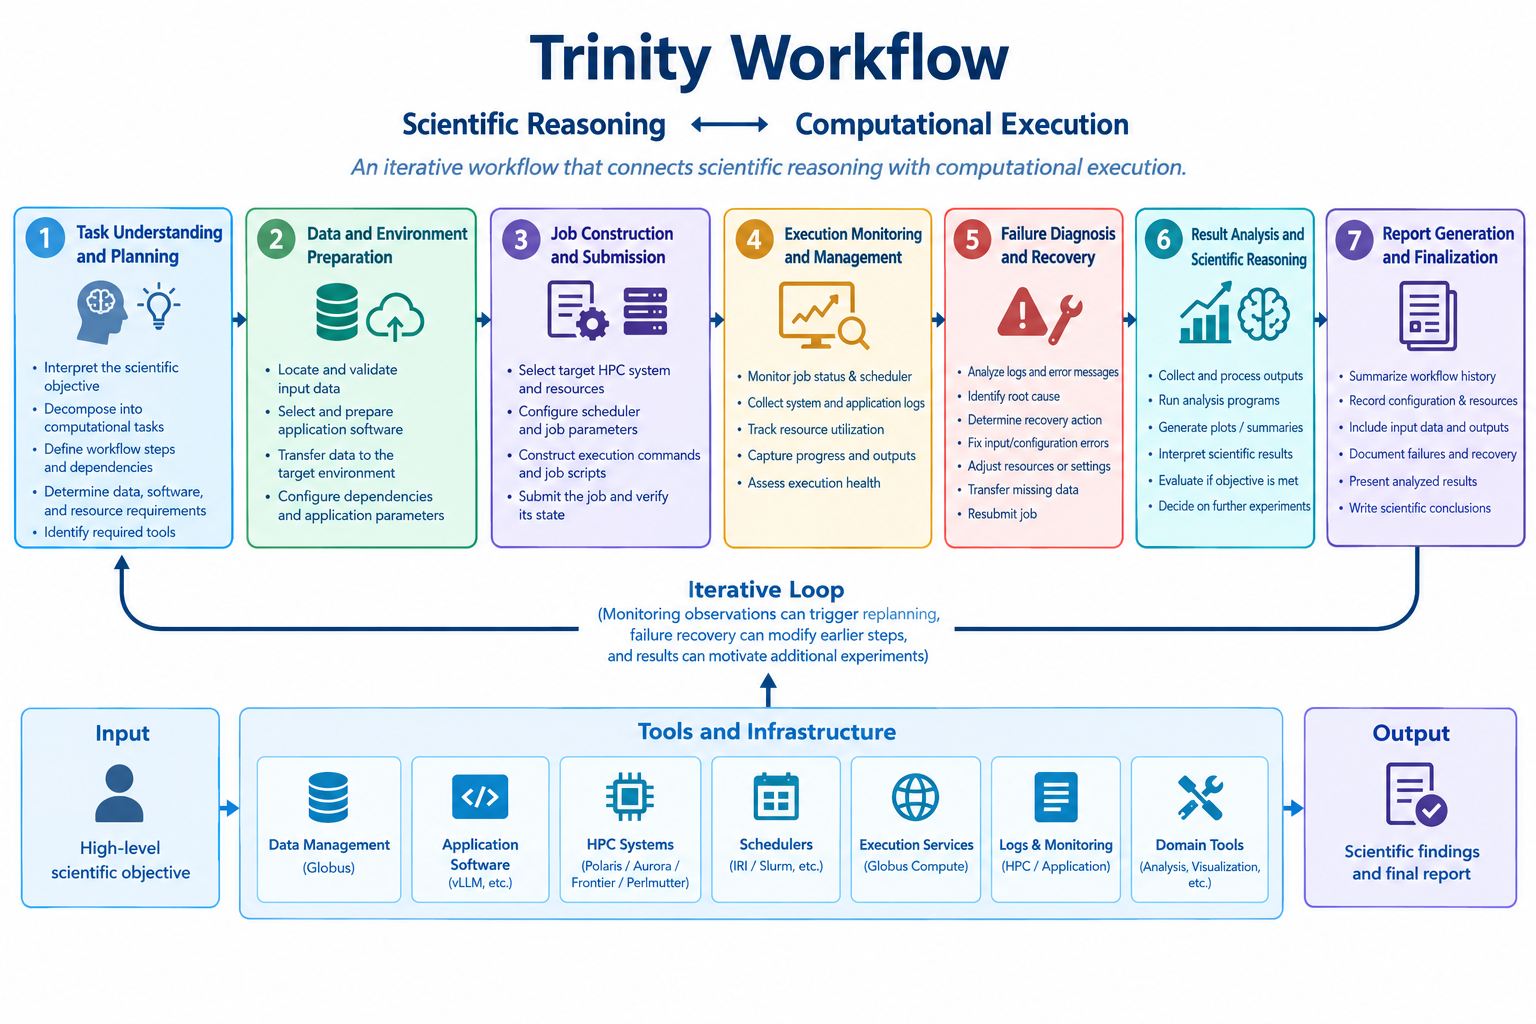
\includegraphics[width=\textwidth,height=0.28\textheight,keepaspectratio]
        {figures/Trinity_Workflow.png}
    \caption{Overview of the Trinity workflow. The four shaded stages---software
    selection, input preparation, resource selection, and batch-job
    creation---are the pre-submission capabilities evaluated in this paper.}
    \label{fig:Trinity_Workflow}
\end{figure*}

The capabilities provided by Trinity are organized into an
iterative workflow, shown in Figure~\ref{fig:Trinity_Workflow}, that
connects \textbf{scientific reasoning with
computational execution}. Given a high-level scientific objective,
the agent determines the computational steps needed to address it,
prepares the required data and software, executes computations on
HPC resources, and reasons over the resulting observations.
Execution is not isolated from reasoning: information collected
during execution can change the agent's understanding of the
workflow state and influence subsequent actions. A workflow may
therefore involve repeated cycles of planning, execution,
monitoring, diagnosis, and scientific reasoning before reaching
a final result.

At a high level, a Trinity workflow consists of
\textbf{task understanding and planning, data and environment
preparation, job construction and submission, execution
monitoring, failure diagnosis and recovery, result analysis and
scientific reasoning, and report generation}. The following
describes each stage and the interactions between them.

\paragraph{Task Understanding and Planning.}
The agent first interprets the user's request to identify the
underlying scientific intent and desired outcome. It decomposes
the objective into computational tasks and establishes a workflow
plan, including the sequence of steps and their dependencies.
The agent also determines the data, software, computational
capabilities, and tools required to carry out the workflow.
At this stage, it identifies requirements rather than committing
to specific input files, software configurations, or HPC resource
allocations. These concrete choices are resolved in subsequent
stages.

\paragraph{Data and Environment Preparation.}
Based on the plan, the agent locates and validates the required
input data, prepares the application software and dependencies,
and configures the execution environment. It may transfer data
to the target computing environment and organize files for
subsequent execution. For workflows involving distributed
resources, the agent can use data-management services such as
Globus to move data between facilities. This stage turns the
workflow's data and software requirements into a usable
computational environment.

\paragraph{Job Construction and Submission.}
With the data and software prepared, the agent determines where
and how to execute the computation. It selects a suitable HPC
system and configures resource requirements, such as the number
of nodes, CPUs, GPUs, memory, and wall time, according to the
application and workflow requirements. The agent then constructs
the job specification, including scheduler parameters, execution
commands, and environment settings. It submits the job through
an HPC execution interface such as IRI or Globus Compute and
verifies that the submission succeeded and that the resulting
execution state is consistent with the planned workflow.

\paragraph{Job Monitoring and Execution Management.}
After submission, the agent observes the execution state and
gathers information needed for subsequent decisions. Monitoring
can include scheduler and job status, HPC system logs, resource
utilization, application logs, execution progress, and generated
outputs. These observations provide both system-level and
scientific context, allowing the agent to determine whether the
computation is progressing normally, has completed, or requires
intervention.

\paragraph{Failure Diagnosis and Recovery.}
Failures are handled as part of the workflow rather than treated
as terminal errors. When an execution step fails or deviates
from expectations, the agent analyzes available evidence,
including scheduler messages, HPC and application logs, error
messages, input data, resource configurations, and previous
workflow actions. It identifies a potential cause and determines
an appropriate recovery action. Depending on the failure,
recovery may involve correcting input or configuration errors,
modifying resource parameters, transferring missing data,
changing execution settings, or resubmitting the job. The
workflow then returns to the relevant preparation, submission,
or monitoring stage.

\paragraph{Result Analysis and Scientific Reasoning.}
Following successful execution, the agent collects and analyzes
the computational results in the context of the original
scientific objective. This stage may involve processing outputs,
running additional analysis programs, generating plots or
summaries, and interpreting application results. The agent
evaluates whether the results sufficiently address the objective
and determines whether additional experiments or computational
steps are necessary. If further work is required, the agent
updates the workflow plan and initiates another execution cycle;
otherwise, it proceeds to report generation.

\paragraph{Report Generation and Finalization.}
Once the agent determines that the scientific objective has been
sufficiently addressed, it consolidates the workflow history and
scientific findings into a final report. The report can include
the original objective, experimental configuration, software and
computational resources, input data, workflow steps, execution
outcomes, failures and recovery actions, analyzed results, and
scientific conclusions. This provides a human-readable record of
both the computational process performed by the agent and the
knowledge obtained from the workflow.

Overall, Trinity combines scientific reasoning with workflow
planning, data and software preparation, HPC resource selection,
tool use, distributed data management, execution monitoring,
failure recovery, and result analysis. The workflow is inherently
iterative: monitoring observations can trigger replanning,
failures can require changes to earlier workflow steps, and
scientific results can motivate additional experiments. This
enables Trinity to move beyond isolated tool invocation toward
end-to-end autonomous execution of complex scientific workflows.



\section{Benchmark Design}\label{sec:benchmark}

\subsection{Benchmark Overview}

The benchmark provides a systematic and reproducible evaluation of the pre-submission capabilities introduced in Section~\ref{sec:introduction}. It is designed around the broader Trinity workflow, while the current instantiation covers four subtasks: software selection, input preparation, resource selection, and batch-job creation. Evaluating each subtask separately matters for a practical reason beyond diagnosis: different stages impose different capability requirements, so a deployment can route the stages a lower-cost model completes reliably to that model and reserve a stronger one for the rest.

\subsection{Benchmark Tasks and Instances}

We define each benchmark instance as a tuple $(\text{subtask}, \text{application}, \text{HPC system})$. Each subtask contains ten instances spanning diverse HPC systems with different architectures, resource configurations, and batch scheduling environments. The benchmark covers representative scientific applications, including molecular dynamics, quantum chemistry, computational fluid dynamics (CFD), LLM inference, and benchmark applications.

The current benchmark evaluates four pre-submission subtasks:

\begin{itemize}
    \item \textbf{Software selection:} identify an appropriate installed application for the described scientific workload.
    
    \item \textbf{Input preparation:} construct the application-specific input artifacts required for a runnable job without inventing unavailable binaries, runtime files, or unsupported inputs.
    
    \item \textbf{Resource selection:} choose the queue, node count, process configuration, and walltime consistent with system constraints and application scaling guidance.
    
    \item \textbf{Batch-job creation:} construct a scheduler script that requests valid resources and invokes the selected application with the prepared inputs.
\end{itemize}

These subtasks are evaluated individually but remain coupled through their dependencies. For example, the selected application determines the required input format and launch command, while the selected resources must be compatible with both the application and the generated batch script.

The complete Trinity workflow extends beyond job construction. After a batch job is created, the agent can submit it through HPC execution infrastructure and monitor scheduler state, system information, application output, and runtime observations. If execution fails, the agent can diagnose the failure, modify the relevant artifact or configuration, and decide whether to resubmit or take another action. If execution succeeds, the agent can retrieve and analyze the results, determine whether the scientific objective has been achieved, and potentially initiate additional computational steps. The workflow concludes with synthesis and reporting of the configuration, execution history, results, and scientific conclusions. The current benchmark isolates the pre-submission stages to provide a controlled evaluation environment, while future extensions will evaluate monitoring, failure diagnosis and recovery, result analysis, scientific reasoning, report generation, and multi-step workflow execution.

\subsection{Domain-Aware Judging}\label{sec:judging}

\begin{figure*}[t]
    \centering
    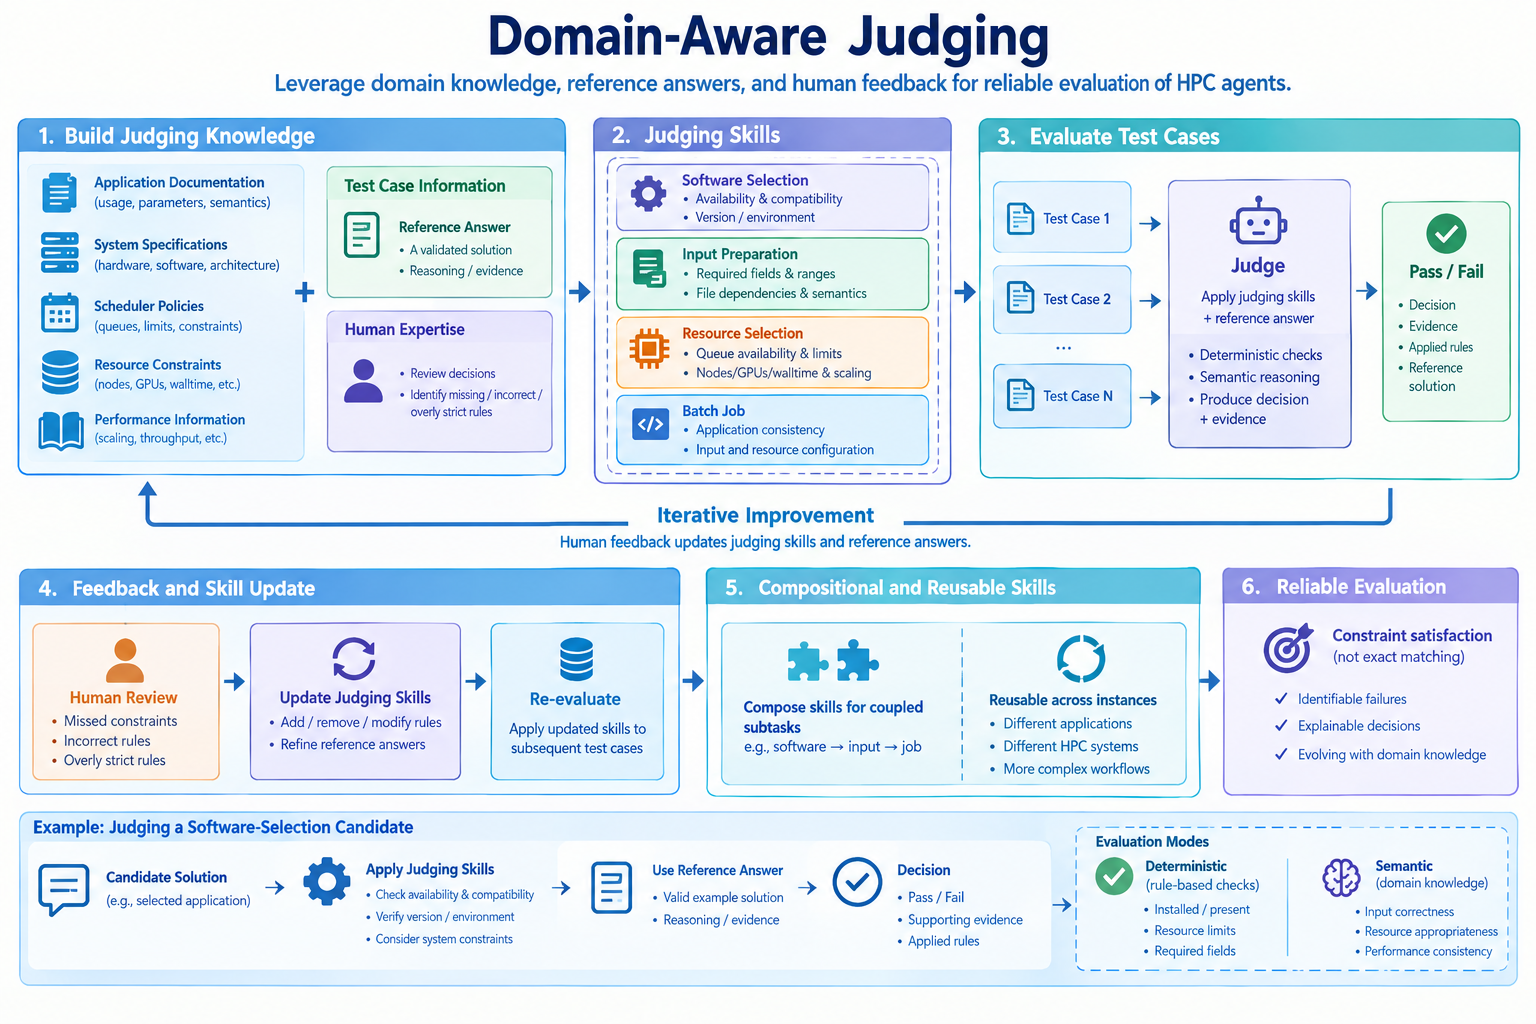
\includegraphics[width=\textwidth,height=0.28\textheight,keepaspectratio]
        {figures/judging.png}
    \caption{Domain-aware judging. Requirements are assembled per instance from a
    versioned library, deterministic checks and semantic judgment produce
    per-requirement verdicts, and scores are derived from those verdicts in code.}
    \label{fig:domain-aware-judging}
\end{figure*}

Correctness here cannot be decided by matching a reference answer, so the judge must be given the constraints explicitly. This subsection describes how those constraints are represented, how a single response is graded against them, and how the library of constraints is revised when a human disagrees with a verdict. Figure~\ref{fig:domain-aware-judging} gives the overall structure; we describe each step in turn.

\subsubsection{Step 1: Rubric assembly}
Requirements live in a library of YAML files organized most-general-first. For one instance the judge loads the root \texttt{\_common} file, then the subtask's \texttt{\_common} file, then an application-specific file where one exists, then the scheduler dialect; later definitions override earlier ones by rule id. Across nine files the library defines 56 requirements. The assembled bytes are hashed, and every grade record stores the rubric identifier and that SHA-256, so grades produced under different rules cannot be silently compared.

\subsubsection{Step 2: The requirement}
Each requirement is a self-contained record naming what must hold, how it is decided, when it applies, and---critically---what evidence supports its existence. Figure~\ref{fig:requirement-yaml} gives the requirement violated in Figure~\ref{fig:motivating-example}, in full.

\begin{figure}[t]
\begin{Verbatim}[fontsize=\scriptsize,frame=single,framesep=2mm]
- id: BATCH.common.filesystems_declared
  claim: "Declares every filesystem the job touches
          with `-l filesystems=`"
  decided_by: deterministic
  check: {kind: regex,
          pattern: '(?m)^\s*#PBS\s+-l\s+filesystems='}
  applies_if: {scheduler: "PBS Pro"}
  dimension: usability
  severity: fatal
  source: "run:138/138"
  support: {runs: 138, of: 138, apps: 6}
  rationale: >-
    ALCF rejects or hangs a job that does not name its
    filesystems. Present in every script of every
    application in the archive - the strongest signal
    in the mined set.
\end{Verbatim}
\caption{One requirement from the library, verbatim. \texttt{source} and
\texttt{support} record the evidence for the rule's existence, not for any
particular verdict; this rule is the one that decides
Figure~\ref{fig:motivating-example}.}
\label{fig:requirement-yaml}
\end{figure}

The \texttt{source} field records provenance in one of four forms: \texttt{run:N/M} (seen in $N$ of $M$ archived successful runs), \texttt{catalog:\textless path\textgreater} (a recorded system or application fact), \texttt{format:\textless spec\textgreater} (an input-format specification), or \texttt{model} (asserted by a language model and not yet confirmed by any run or document). The judge is told this ranking explicitly, so that a rule sourced \texttt{model} is treated as a strong prior rather than a fact.

\subsubsection{Step 3: Free choice}
A requirement is not the only way to be right. Where archived successful runs disagree with one another, that disagreement is itself evidence, and the judge is forbidden from deducting on that axis. The library records 25 such axes across the nine files and injects them into the judge prompt as a separate section. For example, both \texttt{home:eagle} (97 runs) and \texttt{eagle:home} (45 runs) appear in successful scripts, so the ordering of the filesystem list is free, even though the site documentation gives only one ordering. This is the part of the rubric that cannot be derived from a catalog: it requires observing several successful runs of the same code.

\subsubsection{Step 4: Deterministic checks}
Where a rule can be settled mechanically it is: regular expressions over scheduler directives, membership tests against the installed-software table, and numeric comparisons against queue node and walltime limits. A deterministic check has four outcomes, not three---\emph{satisfied}, \emph{violated}, \emph{not applicable}, and \emph{not evaluated}. The fourth is visible rather than silently treated as a pass; a queue-limit check cannot be evaluated when the named queue is absent from the catalog, and recording that explicitly is what prevents a missing fact from being scored as compliance.

\subsubsection{Step 5: Semantic judgment}
The remaining requirements need application or scientific knowledge---whether an input configuration suits the intended workload, or whether a claim contradicts a recorded catalog field. For these the requirement record is handed to the judge verbatim, including its \texttt{claim}, \texttt{rationale}, and \texttt{source}, and the judge returns a verdict with a quoted span of the response as evidence. Where the mechanical test and the requirement's plain claim disagree, the judge is instructed to follow the claim: it is given the mechanism so it can recognize when the mechanism would misfire.

\subsubsection{Step 6: Scores derived in code}
The judge returns verdicts, never scores. Scores are computed from the verdicts in Python: a fatal violation yields 0, a major violation caps the item at 1, and anything else scores 2. This division was adopted after three replicates of the same instance produced three different scores from \emph{identical} verdicts---the judge was reasoning correctly about requirements and arithmetically about totals, and only the latter was unreliable.

\subsubsection{Step 7: Replication}
Every instance is judged $k=3$ times and the per-dimension median is taken. This is a measured necessity rather than a precaution: re-judging identical answers under an identical configuration moved the aggregate pass rate by 2.1 points and flipped 12 of 141 verdicts, with resource selection worst at 21\%. Even at $k=3$, roughly 7\% of rows flip between replicates, and 20 of the 320 instances reported in Section~\ref{sec:eval} are unstable. Differences smaller than about five points are therefore not resolvable by this instrument, and we do not interpret them.

\subsubsection{Step 8: Human review and rule revision}
A human reviews the judge's decisions and can find three kinds of error: a missing constraint, an incorrectly applied rule, or an overly strict rule that rejects a valid solution. Revisions are governed by one rule---\emph{a change that cannot name at least two instances it would fix should not be made}---and every version records its parent, a rationale, and the specific instances motivating each edit.

\begin{table}[t]
\centering
\scriptsize
\caption{Rule revision in practice. Two changes made in the same library version, from the same mining pass over 138 archived production scripts, in opposite directions.}
\label{tab:rule-evolution}
\begin{tabular}{@{}p{0.085\linewidth}p{0.30\linewidth}p{0.50\linewidth}@{}}
\toprule
Change & Rule & Evidence and outcome \\
\midrule
\texttt{add} & \url{BATCH.common.filesystems_declared} & Present in 138 of 138 archived scripts across 6 applications---the strongest signal in the mined set. Added as \emph{fatal}. This is the rule that decides Figure~\ref{fig:motivating-example}. \\
\addlinespace
\texttt{demote} & \url{BATCH.common.cd_workdir} & Written into the site conventions as a rule, and into an earlier rubric as a requirement. Appears in \emph{3 of 138} archived scripts. Enforcing it would fail 98\% of working scripts; demoted to free choice. \\
\addlinespace
\texttt{demote} & \url{BATCH.common.place_scatter} & Proposed by LLM defect-clustering as the highest-reach batch fix (``reaches $\sim$38''). Never universal in any application; demoted to free choice. \\
\bottomrule
\end{tabular}
\end{table}

Table~\ref{tab:rule-evolution} shows why this discipline matters. Rules first derived from site documentation and from LLM clustering of observed defects were wrong in specific, measurable ways, and mining the archive is what exposed them. The same pass that promoted \texttt{filesystems\_declared} to a fatal requirement demoted two rules that documentation and model inference had both endorsed. Later versions applied a reviewer's criterion---\emph{if violating a rule does not stop the script from running, it should not be a requirement}---which removed three cosmetic rules, among them a job-name requirement contradicted by 11 archived scripts that omit \texttt{-N} and ran correctly. Removed rules are retained as comments in the library so that the deletion and its reason remain visible.

One consequence deserves stating plainly, because it cuts against us. The prompts supplied to models still teach two conventions the archive contradicts: they state \texttt{cd \$\{PBS\_O\_WORKDIR\}} as a rule, and give a single filesystem ordering. A model is therefore told one thing and graded by a library that knows better. We resolved this on the judging side only---both appear as free-choice axes and neither is penalized---because regenerating the prompts would have required re-running all four models and invalidated the comparison series mid-experiment.

\begin{table}[t]
\centering
\scriptsize
\caption{Judge output on two instances, verbatim. The judge returns a verdict and a quoted span of evidence for every requirement; scores are derived from the verdicts in code.}
\label{tab:judge-examples}
\begin{tabular}{@{}p{0.17\linewidth}p{0.10\linewidth}p{0.62\linewidth}@{}}
\toprule
Requirement & Verdict & Evidence, and what it means \\
\midrule
\url{filesystems_declared} (fatal) & violated & ``The script has no \texttt{\#PBS -l filesystems=...} directive despite accessing \texttt{/eagle/...} paths.'' \newline \emph{A fatal violation zeroes the item regardless of the other ten requirements, all of which this response satisfied.} \\
\addlinespace
\url{correct_application} (fatal) & violated & ``The authoritative Polaris catalog identifies NWChem, not psi4, as the installed application matching the exact H2O B3LYP/6-31G* 4-MPI-rank benchmark.'' \newline \emph{Psi4 is a real and appropriate quantum-chemistry code; it is simply not installed. Scientific plausibility is not sufficient.} \\
\addlinespace
\url{filesystems_declared} (fatal) & satisfied & ``The script declares \texttt{\#PBS -l filesystems=home:eagle}, covering the Eagle working directory and including home as required by Polaris convention.'' \newline \emph{The judge names the specific directive and why it suffices, so a reviewer can check the verdict rather than trust it.} \\
\bottomrule
\end{tabular}
\end{table}

Table~\ref{tab:judge-examples} shows the resulting output. Because each verdict carries a quoted span, disagreements between a human reviewer and the judge are located at a specific requirement and a specific piece of text, which is what makes the revision loop above tractable.

Finally, the same framework extends to later workflow stages. Requirements for job monitoring, failure diagnosis and recovery, result validation, and reporting can be represented, mined, and revised in exactly this way as the benchmark grows.

\subsection{Open-Weight Models and Inference-Time Capability Augmentation}

\begin{figure*}[t]
    \centering
    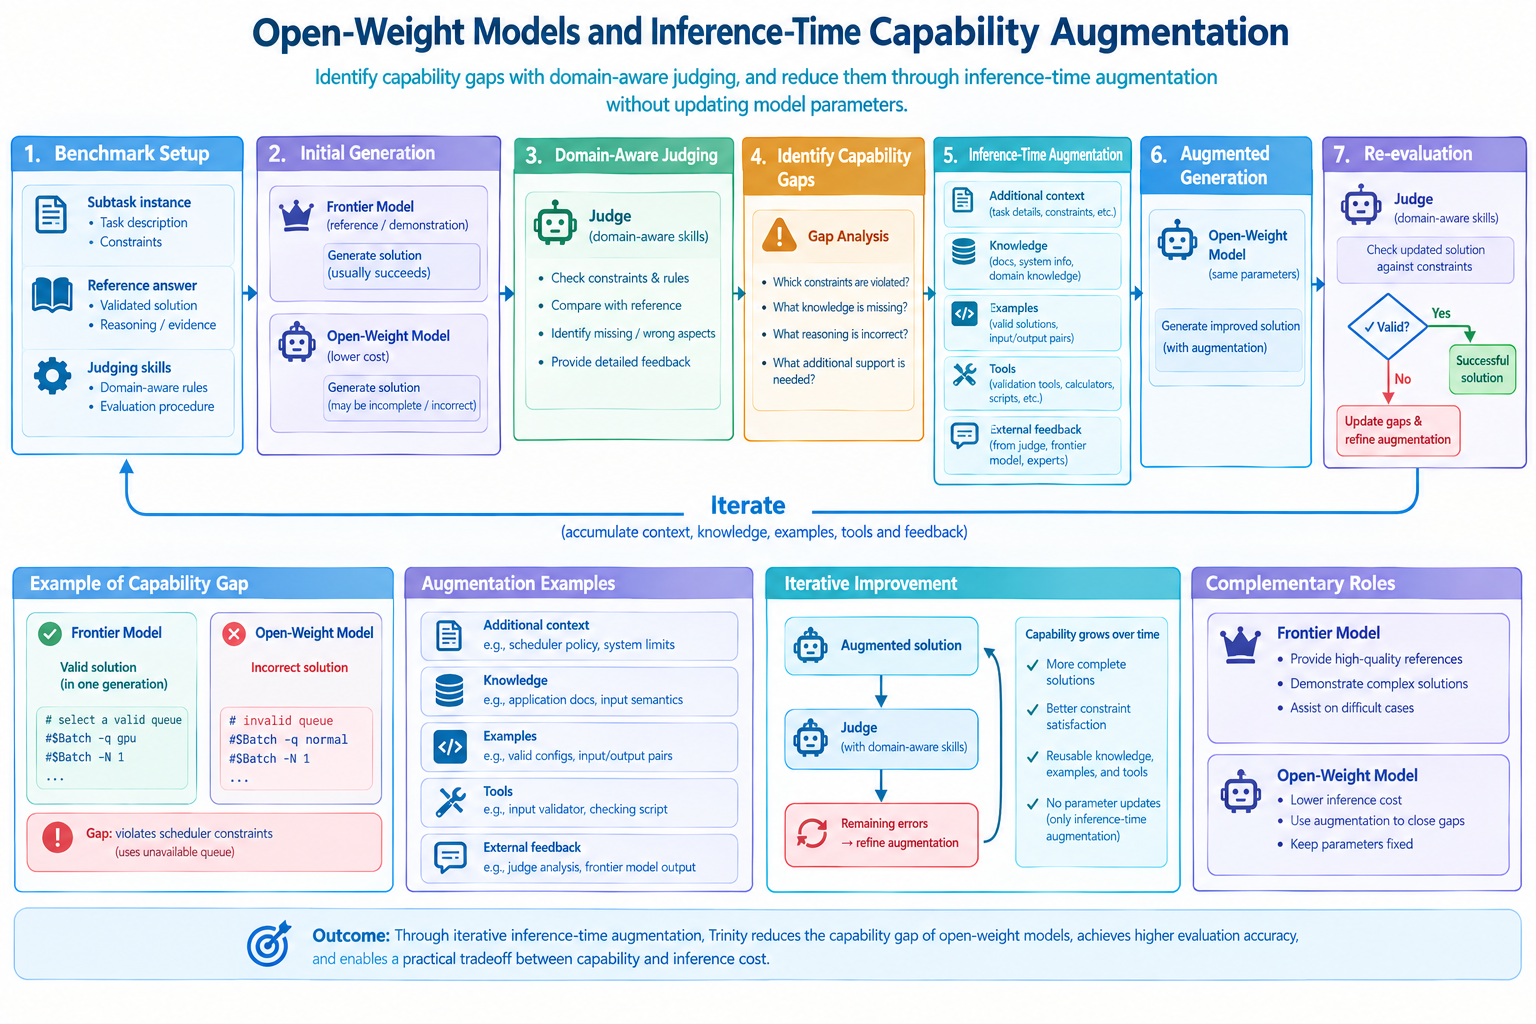
\includegraphics[width=\textwidth,height=0.28\textheight,keepaspectratio]
        {figures/augmentation.png}
    \caption{Inference-time capability augmentation for open-weight models. Judge
    verdicts identify which constraint was not satisfied; the corresponding
    context, knowledge, or examples are supplied in the prompt and the instance is
    re-attempted, with model parameters unchanged.}
    \label{fig:augmentation}
\end{figure*}

Open-weight models are a lower-cost alternative to frontier models but may be weaker on complex scientific and HPC tasks. As Figure~\ref{fig:motivating-example} illustrates, some of that weakness is not a reasoning deficit at all but a missing site-specific fact, and such gaps can be closed without touching the model parameters. Figure~\ref{fig:augmentation} shows the loop: the judge reports \emph{which} requirement failed and why, the corresponding context, knowledge, or example is added to the prompt, and the instance is attempted again. Because each verdict names a requirement rather than reporting a score, the feedback is specific enough to act on---an invalid queue points to the queue table, an invented input keyword points to the format specification, a malformed directive points to the site's scheduler conventions.

\textbf{Prompt arms.} To measure this effect we define prompt arms that differ only in how much facility knowledge they carry, derived from a single source text so the contrast is exact:

\begin{itemize}[leftmargin=*,itemsep=1pt,topsep=2pt]
\item \textbf{\texttt{bare}}---the task, the workload, and the output contract, plus only those instructions that stand alone. The installed-software listing, required-file inventory, module lines, site scheduler conventions, and worked examples are removed, as are any instruction clauses that refer to removed material.
\item \textbf{\texttt{rich}}---the full prompt: catalog facts, site conventions, worked examples, and, for input preparation, explicit format contracts and scaling notes.
\end{itemize}

The two are produced from the same base prompt by deletion and insertion respectively, and the transformation is verified to be byte-reversible. Deletion is deliberately conservative: the workload itself, the pipeline carry-forward, the charge account, and the scheduler name are always retained, because they define the task rather than supply its answer. Exactly one non-deletion edit is applied and recorded---``consult the system's software catalog and identify'' becomes ``Identify''---so that removing a block never leaves a dangling reference. Every removed block is recorded per instance, which is what allows the augmentation in Figure~\ref{fig:motivating-example} to be quoted exactly.

Two properties of this design matter when reading the results. First, the arms differ in supplied \emph{knowledge}, not in task difficulty: the grading key is identical. Second, the \texttt{rich} arm's additions beyond the base prompt apply only to input preparation, so roughly three quarters of the corpus is byte-identical between them and serves as a built-in noise control.

Whether a gain is a real capability improvement or merely the prompt supplying the answer cannot be settled by the aggregate pass rate, and Section~\ref{sec:knowledge-split} reports the measurement we registered in advance to separate the two.

\section{Experimental Evaluation}
\label{sec:eval}
 
\subsection{Experimental Setup}
We evaluate four open-weight models on the proposed HPC agent benchmark: Nemotron-3-Ultra, Gemma-4-31B, GPT-OSS-120B, and Llama-3.1-8B. They span a range of sizes and capabilities and let us examine whether lower-cost models can reliably perform individual stages of an HPC workflow.

The evaluation uses ten benchmark instances for each of the four pre-submission subtasks, giving 40 instances. Each instance is attempted under both prompt arms, producing 20 attempts per model per subtask and 320 model responses in total. Every response is graded three times (Section~\ref{sec:judging}, Step 7), for 960 judgments per arm. A response passes a subtask only if it violates no fatal and no major requirement; each violation is recorded with its severity and the judge's quoted evidence, giving both an aggregate success measure and a fine-grained view of failure modes. Each model is called once per instance through a chat completion interface with a single user message: no system prompt, no tools, no retrieval, no filesystem access and no second attempt. A model cannot consult application documentation, run a parser, or observe a failure and revise. Every number below is therefore unaided one-shot performance and should be read as a lower bound on what an agent with tool access would achieve.

\textbf{Why the judge is a different model family from the author.} The benchmark prompts and their reference answers are written by Claude (Section~\ref{sec:generation}). Using Claude again as the judge would close the loop, with one model family writing the question, the answer key, and the grade; a rubric error and a generation error would then be correlated in a way no measurement could detect. We therefore judge with a GPT model, \texttt{gpt-5.6-terra}, accessed through the facility's internal API. It was selected as the strongest available GPT model and the best performer on this benchmark (61\% answer-correct, 46\% fully correct over 156 samples), on the reasoning that judging competence is at least bounded below by task competence.

This choice moves a bias rather than eliminating it, and we state the residual risk explicitly: GPT-OSS-120B is one of the graded models and the judge is a GPT model, so judge self-preference is possible and \emph{we have not measured it}. GPT-OSS-120B scores second-lowest of the four, which is the wrong direction for the obvious bias but is not a measurement. The infrastructure for the measurement exists---the judging interface is model-agnostic and a cross-judge design that varies one factor per cell is specified---but the cross-judge comparison has not been run, and no claim in this paper should be read as depending on its outcome.

\textbf{Rubric version.} The judgments were collected under rubric version r27 and are reported here under r28, which retires one input-preparation rule. The rule penalized responses for resembling the worked example the prompt itself supplied; it fired on 18 of 40 input-preparation instances and was a false positive in roughly three quarters of them, flagging conventional values---a standard LAMMPS bin skin, a tutorial's port number, solver defaults---and, in one case, a header that another rule in the same library requires fatally. Because scores are derived from per-requirement verdicts in code rather than produced by the judge (Step 6), retiring a rule can be replayed offline against verdicts already collected: the judge was asked the same questions and the retired one is simply not counted. This avoids both the cost of 960 further judge calls and the fresh sampling noise they would introduce. Replaying rather than re-judging is only valid for changes that remove rules or relax severities, and the replay tool refuses to score any rubric containing a rule for which the corpus holds no verdict.

\subsection{Benchmark Sample Generation}\label{sec:generation}
Each benchmark instance is generated by a frontier model, \texttt{claude-sonnet-4-6}, from a structured specification rather than written free-form. A single call returns both the prompt and its reference answer, conditioned on the real catalog entry for the target system and application, so that the reference agrees with the recorded module lines, input types, queue names, and build defaults.

\textbf{Instance space.} An \emph{anchor} is a (domain, application, system) triple; 39 anchors are defined, restricted to application/system pairs confirmed to be installed and executable. Crossing four subtasks with all anchors gives 156 possible instances, of which this paper reports a frozen stratified subset of ten anchors, one instance per subtask, for 40 instances. The subset is chosen rather than sampled so that a 40-instance run still spans what varies: all seven systems, both scheduler families (PBS Pro and Slurm), ten applications across ten scientific domains, and---because the effect of a worked example on input preparation is one of the things being measured---three anchors with a verified upstream input deck and seven without. Two anchors are deliberately sparse and act as a placebo stratum. A situational \emph{variation} (for example, ``a deadline run where turnaround matters most'') is assigned deterministically per instance, offset by subtask so that the same anchor meets a different situation at each stage.

\textbf{Preventing answer leakage.} The governing instruction to the generator is to state the task explicitly but never reveal the answer, and compliance is enforced rather than assumed. Each subtask carries a list of forbidden terms that would pre-empt a \emph{downstream} subtask's answer---application names, resource expressions such as \texttt{select=} or \texttt{mpiexec -n}, and scheduler tokens such as \texttt{\#PBS} or \texttt{module load}. Term matching alone proved insufficient, because a prompt can state the conclusion in fluent English without using any forbidden token; a further 14 regular expressions catch constructions such as ``a single node is sufficient'' or ``the \emph{X} queue is the right choice.'' A generated sample that trips either check is regenerated, with the offending terms quoted back to the generator, up to three attempts; samples that still leak are recorded as such and excluded. Because some blocks are \emph{deliberately} supplied---the software catalog necessarily contains the correct application's name---the scan exempts those blocks specifically, while any mention of the same terms elsewhere in the prompt still counts as a leak.

\textbf{Pre-generation gates.} Six automated checks run before generation is allowed, of which two are worth naming because they guard against silent failure rather than visible error. A \emph{redaction gate} requires the input-scaling filter to be observed firing, on the principle that a filter that never runs and a filter that works are indistinguishable from their output alone. A \emph{negative control} scores a block against the wrong subtask's terms and fails if it comes back clean, which would indicate an empty or malformed block passing every other check. A coherence gate over all 39 anchors caught a substantive defect in an earlier corpus: one anchor's carry-forward named a queue that does not exist on the target system, and all four models obeyed the prompt and were failed fatally for it.


\subsection{Judging Requirements by Subtask}\label{sec:rubric-detail}
Table~\ref{tab:rubric} summarizes the judging requirements used for each subtask, including their number, severity, and decision method. Each requirement has one of three severity levels. A \emph{fatal} violation assigns a score of 0 regardless of the other requirements; a \emph{major} violation caps the item at 1 out of 2; and a \emph{minor} violation does not prevent the maximum score of 2. Requirements also differ in how they are evaluated. \emph{Deterministic} requirements are checked programmatically against recorded facts, such as an installed-software table, queue node and walltime limits, or the scheduler dialect. \emph{Judge-decided} requirements require semantic assessment of the response, such as determining whether a claim contradicts the catalog or whether a value is consistent with the specified physical system.
\begin{table}[t]
\centering
\caption{Requirements loaded per subtask, by severity and decision method}
\label{tab:rubric}
\begin{tabular}{lccccc}
\toprule
Subtask & Reqs. & Fatal & Major & Minor & Judge \\
\midrule
Software selection & 4 & 1 & 2 & 1 & 2 \\
Input preparation & 25 & 13 & 12 & 0 & 6 \\
Resource selection & 10 & 3 & 6 & 1 & 4 \\
Batch-job creation & 17 & 8 & 8 & 1 & 1 \\
\midrule
Total & 56 & 25 & 28 & 3 & 13 \\
\bottomrule
\end{tabular}
\end{table}
The four subtasks differ substantially in the structure of their requirements. \emph{Input preparation} has the largest rubric, with 25 of the 56 requirements, including 13 fatal requirements. These rules capture concrete properties of application input artifacts, such as required files, mandatory sections, valid keywords, and physical parameter values; 19 of the 25 requirements are therefore evaluated deterministically against the corresponding input-format contract. \emph{Batch-job creation} is similarly dominated by deterministic checks: 16 of its 17 requirements can be evaluated against system and scheduler specifications, including queue availability, walltime limits, node requests, scheduler syntax, and application invocation.
\emph{Resource selection} contains 10 requirements, four of which require judge-based semantic assessment. These include whether resource choices are consistent with the workload and whether supporting claims are appropriately grounded. \emph{Software selection} has the smallest rubric, with four requirements, two of which require semantic judgment. Its requirements focus on selecting the appropriate application and accurately describing its capabilities and availability, rather than requiring exhaustive reproduction of catalog information.
Across all four subtasks, 43 of the 56 requirements (77\%) are evaluated deterministically, while only 13 (23\%) require semantic judgment. Thus, the rubric relies primarily on reproducible checks against recorded application and system facts, while using semantic judgment for cases where exact matching is insufficient. Table~\ref{tab:rule-list} lists all 56 requirements and their severity by subtask. The complete definition of each rule---including its claim, decision method, and rationale---is released as a versioned artifact alongside the benchmark.
\begin{table}[t]
\centering
\scriptsize
\caption{All 56 judging requirements by subtask (superscript: F = fatal, M = major, m = minor)}
\label{tab:rule-list}
\begin{tabular}{@{}p{0.13\linewidth}p{0.83\linewidth}@{}}
\toprule
Subtask & Requirements \\
\midrule
Software (4) & \url{names_one_application}$^{M}$, \url{no_vague_performance_claims}$^{m}$, \url{correct_application}$^{F}$, \url{claims_true_to_catalog}$^{M}$ \\
Input prep. (25) & \url{all_required_files_present}$^{F}$, \url{mandatory_sections_present}$^{M}$, \url{file_identifiable}$^{M}$, \url{exact_filenames_used}$^{M}$, \url{no_output_as_input}$^{M}$, \url{no_binary_contents}$^{F}$, \url{no_truncation}$^{M}$, \url{no_invented_keywords}$^{F}$, \url{values_match_physical_system}$^{M}$, \url{gromacs.tpr_not_authored}$^{F}$, \url{gromacs.grompp_step_stated}$^{M}$, \url{gromacs.mdp_keys_real}$^{F}$, \url{gromacs.required_mdp_fields}$^{M}$, \url{hpl.positional_format}$^{F}$, \url{hpl.header_and_output_lines}$^{F}$, \url{hpl.count_lines_match}$^{F}$, \url{hpl.grid_matches_ranks}$^{M}$, \url{qe.namelist_syntax}$^{F}$, \url{qe.required_namelists}$^{F}$, \url{qe.required_cards}$^{F}$, \url{qe.nat_matches_positions}$^{F}$, \url{qe.ntyp_matches_species}$^{F}$, \url{qe.no_card_terminator}$^{M}$, \url{qe.ibrav_consistent}$^{M}$, \url{qe.pseudopotentials_plausible}$^{M}$ \\
Resource sel. (10) & \url{queue_exists}$^{F}$, \url{no_reservation_queue}$^{M}$, \url{nodes_within_queue_limits}$^{F}$, \url{walltime_within_queue_limit}$^{F}$, \url{ranks_match_build_defaults}$^{M}$, \url{rank_layout_plausible}$^{M}$, \url{rank_arithmetic_consistent}$^{M}$, \url{no_fabricated_evidence}$^{M}$, \url{allocation_matches_scaling_notes}$^{m}$, \url{sizing_not_absurd}$^{M}$ \\
Batch job (17) & \url{filesystems_declared}$^{F}$, \url{walltime_declared}$^{F}$, \url{queue_declared}$^{F}$, \url{select_declared}$^{M}$, \url{account_declared}$^{M}$, \url{queue_exists}$^{F}$, \url{correct_dialect}$^{F}$, \url{no_directive_comments}$^{M}$, \url{invokes_application}$^{F}$, \url{no_placeholders}$^{F}$, \url{inputs_reachable}$^{M}$, \url{slurm.walltime_declared}$^{F}$, \url{slurm.account_declared}$^{M}$, \url{slurm.queue_or_qos_declared}$^{M}$, \url{slurm.nodes_declared}$^{M}$, \url{slurm.no_directive_comments}$^{m}$, \url{slurm.srun_launcher}$^{M}$ \\
\bottomrule
\end{tabular}
\end{table}

\subsection{Results}\label{sec:results}

\begin{table}[t]
\centering
\caption{Instances passed, by model and subtask, under both prompt arms. A pass requires no fatal and no major violation, at the median of three judgments. Each cell is out of 10; each row total is out of 40.}
\label{tab:main-results}
\setlength{\tabcolsep}{4pt}
\begin{tabular}{lcccc@{\hskip 8pt}c}
\toprule
Model & Software & Input & Resource & Batch & Total \\
\midrule
\multicolumn{6}{l}{\emph{\texttt{bare} --- facility knowledge removed}} \\
Nemotron-3-Ultra & 4 & 2 & 2 & 1 & 9/40 \\
Gemma-4-31B      & 5 & 2 & 2 & 0 & 9/40 \\
GPT-OSS-120B     & 4 & 0 & 1 & 0 & 5/40 \\
Llama-3.1-8B     & 3 & 0 & 1 & 0 & 4/40 \\
\cmidrule(l{-2pt}r{2pt}){1-6}
All models & 16/40 & 4/40 & 6/40 & 1/40 & \textbf{27/160} \\
\midrule
\multicolumn{6}{l}{\emph{\texttt{rich} --- full facility context}} \\
Nemotron-3-Ultra & 8 & 4 & 9 & 10 & 31/40 \\
Gemma-4-31B      & 8 & 3 & 9 & 8  & 28/40 \\
GPT-OSS-120B     & 4 & 3 & 10 & 5 & 22/40 \\
Llama-3.1-8B     & 9 & 0 & 3 & 6  & 18/40 \\
\cmidrule(l{-2pt}r{2pt}){1-6}
All models & 29/40 & 10/40 & 31/40 & 29/40 & \textbf{99/160} \\
\bottomrule
\end{tabular}
\end{table}

Table~\ref{tab:main-results} reports the main result. Without facility knowledge every model performs poorly---27 of 160 instances passed in aggregate, with batch-job creation almost unsolved at 1 of 40. Supplying that knowledge raises the aggregate to 99 of 160. The ordering of models is stable across arms at the top and bottom, but the gains are not uniform: Nemotron-3-Ultra gains 22 instances and Llama-3.1-8B only 14, and the two middle models change places.

The gains are concentrated where the missing information was site-specific. Batch-job creation improves from 1/40 to 29/40 and resource selection from 6/40 to 31/40, while input preparation improves only from 4/40 to 10/40 and remains the weakest subtask for every model. At the requirement level the pattern is sharper still: the filesystem directive of Figure~\ref{fig:motivating-example} goes from 31 violations to none, \texttt{queue\_exists} from 18 to none, \texttt{nodes\_within\_queue\_limits} from 27 to 3, and \texttt{ranks\_match\_build\_defaults} from 27 to 4. Each corresponds directly to a fact the augmented prompt supplies---the per-queue node limits, the required filesystem list, the build's default rank count.

We report pass/fail rather than violation counts as the endpoint, and the requirement-level counts above should be read as illustrative only. Violation counts systematically understate the unaugmented arm, because a check returns \emph{not evaluated} rather than \emph{violated} when the fact it needs is absent: a bad queue name costs one violation when the queue table is missing and three when it is present. Pass/fail is unaffected by this censoring.

\textbf{What augmentation does not fix.} Several failure modes persist with the relevant information explicitly in the prompt, and these are the more informative results. One class is not among them, and we correct it here rather than let it stand: both Nemotron-3-Ultra and GPT-OSS-120B claim GPU offload for the Quantum ESPRESSO build on Aurora---``Intel Xe GPU (XPU) accelerators via SYCL/DPC++ offload''---against a catalog that records \texttt{gpu\_support: false}. That field is graded but was \emph{never rendered into any prompt}, in any arm, so this is not a model contradicting supplied context. Section~\ref{sec:withheld} reports what happens when it is supplied. The remaining modes are genuine. Some are arithmetic rather than informational: Gemma-4-31B writes a QE cell with \texttt{celldm(1)=10.26}, a 5.43\,\AA{} primitive cell, when the requested structure is an 8.716\,\AA{} $2\times2\times2$ supercell, and produces a GROMACS ion count corresponding to 0.27\,M NaCl against a 0.15\,M target. Llama-3.1-8B specifies 128 ranks at one GPU per rank while the request requires two. A third kind is procedural: GPT-OSS-120B continues to append explanatory comments to \texttt{\#PBS}/\texttt{\#SBATCH} directive lines on 4 of 10 batch instances despite the scheduler conventions stating that PBS reads trailing text as a further directive, and Llama-3.1-8B invokes AlphaFold as \texttt{srun ... python .../bin/python run\_alphafold.py}, using one Python interpreter to execute another as a script.

Input preparation is the clearest capability gap. It is the largest rubric, it is the only subtask where augmentation changes little, and its residual failures are application-semantic rather than site-specific: invented configuration keywords such as a NekRS \texttt{[STATISTICS]} block, a lowercase \texttt{targetWalkers} in a case-sensitive QMCPACK field, and---for Llama-3.1-8B, which passes none of the ten instances under either arm---substitution of an invented single input file for the \texttt{.par}, \texttt{.re2}, and \texttt{.udf} artifacts the application requires.

\subsection{Separating Supplied Knowledge from Capability}\label{sec:knowledge-split}

\begin{table}[t]
\centering
\caption{Pass rates when scoring is restricted to requirement classes registered before any answer was collected. \emph{Knowledge}: satisfiable from what a competent model already knows. \emph{Supplied}: depends on a fact appearing only in the injected material. \emph{Mixed}: arguable, never folded into either.}
\label{tab:knowledge-split}
\setlength{\tabcolsep}{5pt}
\begin{tabular}{lcccc}
\toprule
Scoring view & Rules & \texttt{bare} & \texttt{rich} & Gain \\
\midrule
All requirements   & 56 & 27/160 \ (17\%) & 99/160 \ (62\%) & +45\,pp \\
Knowledge only     & 39 & 87/160 \ (54\%) & 119/160 (74\%) & +20\,pp \\
Knowledge + mixed  & 45 & 63/160 \ (39\%) & 104/160 (65\%) & +26\,pp \\
Supplied only      & 11 & 80/160 \ (50\%) & 148/160 (92\%) & +42\,pp \\
\bottomrule
\end{tabular}
\end{table}

A 45-point gain from adding context invites an obvious objection: the facts were deleted from the prompt and the models were then graded on those same facts. The symmetric objection applies to the obvious remedy---scoring only the knowledge-independent requirements removes precisely the rules that decide most instances. Neither can be answered after the fact by choosing whichever subset is favorable, so every one of the 56 requirements was classified in advance, on 2026-09-23, before a single answer in this experiment was collected, as \emph{knowledge} (39), \emph{supplied} (11), or \emph{mixed} (6). The classification is a second aggregation of the same verdicts, never a re-judge.

Table~\ref{tab:knowledge-split} reports all four views. The headline gain of 45 points falls to 20 points when scoring is restricted to requirements a competent model could satisfy unaided, and the supplied-only view moves 42 points to near-saturation (92\%). Read together, these say that the majority of the aggregate improvement is the prompt supplying facts the model could not have known, exactly as the objection supposes---and that a real, smaller improvement survives that correction. Both readings are true, and reporting only one of them would misrepresent the result.

Two caveats belong with this table. First, the split is \emph{not interpretable at all} for software selection, and more strongly than a thin-column warning conveys: that stage has no requirements in the \emph{supplied} class, and its two \emph{knowledge} requirements are a formatting check no model fails and a \emph{minor} that cannot block a pass. Both columns therefore score nothing in either arm, and the stage's entire contribution falls in \emph{mixed}. We report software selection at all-rules only and draw no knowledge/capability conclusion from it. Section~\ref{sec:withheld} sharpens this: once the withheld field is rendered, the requirement that fires on it is contradicting a fact printed in the prompt---a supplied-knowledge failure by any reading---yet the registered classification still calls it arguable, and the stage moves from 66/78 to 75/78 with zero movement in either the knowledge or the supplied column. We have deliberately not reclassified it. The classification's value rests on having been fixed before any answer was collected, and amending it to fit results obtained afterwards would forfeit exactly that; the revision is recorded against the artifact and applies from the first corpus in which the field is supplied. Second, the unaugmented arm's knowledge-only pass rate (54\%) is far above its all-rules rate (17\%), which is the expected consequence of removing rules that a withheld fact makes unsatisfiable, not evidence that the models are stronger than Table~\ref{tab:main-results} suggests.

\subsection{When a Graded Fact Is Never Supplied}\label{sec:withheld}

Section~\ref{sec:knowledge-split} measures how much of the augmentation gain comes from facts the prompt supplies. A sharper version of that question is whether the benchmark ever grades a fact it does \emph{not} supply. It did, and this subsection reports the consequence.

\texttt{SOFT.common.claims\_true\_to\_catalog} evaluates an answer against the catalog's \texttt{gpu\_support} field. That field appeared in \emph{none} of the 200 prompts across any arm: the catalog block shown to the model was rendered from an application's name and a truncated description, and no other field. The judge received it; the model never did. The effect was concentrated and stable---two models were violated 3/3 on Quantum ESPRESSO on Aurora in all three arms, eighteen runs out of eighteen, while selecting the correct application every time. Across the corpus, 51 of 56 violations of this requirement fall on responses whose application choice is correct.

\textbf{Design.} We constructed three prompt arms over 39 anchors and two models, derived from a common base by textual insertion rather than regeneration, and verified byte-reversible. \texttt{fieldbool} adds \texttt{[gpu\_support: true|false]} to each catalog line; \texttt{fieldprose} adds \texttt{[GPU-accelerated build]} or \texttt{[CPU-only build; no GPU offload]}; \texttt{contract} adds no fact and instead instructs the model to assert only properties the catalog records. The first two carry identical information and differ only in wording, so presentation is priced separately from content. The primary endpoint was fixed before the numbers were read: the requirement satisfied, on the 12 anchors recording \texttt{gpu\_support: false} (24 cells), paired against base with an exact McNemar test. The 26 anchors recording \texttt{true} (52 cells) control against inducing the opposite error, and \texttt{correct\_application} over all 78 cells is a guard rail, because an earlier instruction of the \texttt{contract} arm's shape had regressed application choice.

\begin{table}[t]
\centering
\scriptsize
\caption{Capability arms, paired against base, exact McNemar. Primary endpoint is the treated column; controls and guard rail are reported alongside because a treatment that fixes one and breaks another has not helped.}
\label{tab:withheld}
\setlength{\tabcolsep}{3.5pt}
\begin{tabular}{lccccccc}
\toprule
arm & treated & fixed & broke & $p$ & controls & guard & vague \\
    & (24) & & & & (52) & \url{corr_app} & claims \\
\midrule
\texttt{fieldbool}  & 18$\to$\textbf{24} & 6 & 0 & \textbf{0.031} & 52$\to$52 & 72$\to$75 & 61$\to$64 \\
\texttt{fieldprose} & 18$\to$23 & 6 & 1 & 0.125 & 52$\to$50 & 72$\to$72 & 61$\to$64 \\
\texttt{contract}   & 18$\to$23 & 5 & 0 & 0.062 & 52$\to$51 & 72$\to$74 & 61$\to$\textbf{74} \\
\bottomrule
\end{tabular}
\end{table}

\textbf{Results.} Table~\ref{tab:withheld} reports them. Rendering the field as a boolean eliminates every treated violation and breaks nothing, with no movement on the controls and no regression in the guard rail; stage pass rate goes from 66/78 to 75/78. The terse machine-readable form outperformed prose, which fixed the same six and broke three elsewhere. Note that $p=0.031$ sits exactly on the achievable floor: six one-directional flips is the minimum that clears $0.05$ at 24 cells, and five would not have.

Two results were not the object of the experiment and are reported because they bear on Section~\ref{sec:knowledge-split}. The \texttt{contract} arm moved \texttt{no\_vague\_performance\_claims} from 61/78 to 74/78---13 fixed, 0 broken, $p=0.0002$---the one requirement that never improved with added context in the main ablation. An instruction repaired what more information could not. And \texttt{contract} induced a new failure mode: models reporting that the catalog is silent about a property and being marked wrong, because the judge holds a field the model was never shown. That is the defect this subsection documents, reproduced by an intervention designed to encourage honesty about uncertainty.

\textbf{Interpretation.} Only about a third of the 85\%$\to$96\% stage improvement is attributable to the pre-registered endpoint; the rest is unregistered movement that would need its own experiment to claim. We report 18$\to$24 as the result and the pass-rate change as context. More broadly this is a benchmark-construction finding rather than a model-capability one, and it is mechanically detectable: every field a rubric can fire on should appear in the rendered prompt, or the rubric should not fire on it. These arms use a separate corpus and are not comparable to Table~\ref{tab:main-results}.

\subsection{Discussion}
Three properties of these results generalize beyond the specific models evaluated.

\textbf{Capability is stage-dependent, so a single aggregate score is misleading.} The same model can construct valid scheduler scripts at 10/10 and prepare valid application inputs at 4/10. Reporting one number per model would hide that, and it is the per-stage view that makes the practical consequence visible: stages differ enough in difficulty that routing them to different models is a reasonable deployment strategy, which is not a conclusion an end-to-end benchmark could support.

\textbf{Most failures are constraint violations, not generation errors.} The responses in Figure~\ref{fig:motivating-example} are fluent, well-formed, and plausible under both arms; what separates them is a single directive. Textual quality is therefore uninformative here, and evaluation has to be grounded in constraints that reflect what the target system actually requires. Grounding those constraints in archived production runs rather than documentation was not a refinement but a correction---documentation-derived rules were measurably wrong (Table~\ref{tab:rule-evolution}).

\textbf{Measuring augmentation requires separating supplied knowledge from capability, and the separation must be registered in advance.} The same experiment supports ``context improves pass rates by 45 points'' and ``by 20 points'' depending on which requirements are scored, and both are defensible readings of the same verdicts. Committing to the classification before collecting answers is what makes the pair of numbers evidence rather than a choice. We would expect this to be a general requirement for prompt-augmentation studies in domains where the prompt can carry the answer, which describes most facility-specific settings.

The most useful negative result is input preparation. It is the one stage augmentation does not repair, its residual failures are application-semantic rather than site-specific, and it is where retrieval of application documentation, format validation tools, and iterative refinement against a validator would be expected to help---mechanisms this experiment deliberately did not include, since it varies only prompt content with parameters and tooling fixed.

\section{Conclusion}\label{sec:conclusion}

We presented \textit{Trinity}, a multi-agent framework connecting LLM-based reasoning with scientific applications, HPC systems, execution infrastructure, and scientific feedback, together with a benchmark for four foundational pre-submission capabilities: software selection, input preparation, resource selection, and batch-job creation. The benchmark evaluates constraint satisfaction rather than textual similarity, using a versioned requirement library mined from archived production runs, in which disagreement among successful runs is recorded as free choice the judge may not penalize.

Across 320 responses from four open-weight models, supplying facility knowledge in the prompt raises pass rates from 27/160 to 99/160. Restricted to requirements classified in advance as satisfiable without that knowledge, the same augmentation yields 87/160 to 119/160---so most, but not all, of the apparent gain is the prompt supplying facts the models could not have known. Input preparation is the capability gap augmentation does not close, and it fails for application-semantic rather than site-specific reasons.

Two limitations bound these conclusions. Judge self-preference is unmeasured: one graded model shares a family with the judge, and although it scores second-lowest, the cross-judge comparison has not been run. And the benchmark's resolution is limited by judge variance to roughly five points, so the ordering of adjacent models should not be over-read. Future work will run that comparison, extend the benchmark to execution monitoring, failure diagnosis, result analysis, and scientific reasoning, and evaluate the richer inference-time mechanisms---retrieval, validation tools, and iterative refinement---that the input-preparation gap most clearly calls for.


% ============================================================
% Acknowledgments
%
% DO NOT include identifying information in the double-anonymous
% submission. Add acknowledgments only in the appropriate
% camera-ready version.
% ============================================================

% \section*{Acknowledgment}
% [Acknowledgments for camera-ready version.]


% ============================================================
% References
% ============================================================

\bibliographystyle{IEEEtran}
\bibliography{references}

\end{document}
